\documentclass[9pt,conference]{IEEEtran}

\usepackage[pdftex]{graphicx}
\usepackage{url}

\begin{document}

\title{Designing an Actor Model Game Architecture with Pony}

\author{\IEEEauthorblockN{Nick Pr\"uhs}
\IEEEauthorblockA{Daedalic Entertainment\\
Hamburg, Germany\\
nick.pruehs@daedalic.com}}

\maketitle

\begin{abstract}
Pony is an open-source, object-oriented, actor-model, capabilities-secure,
high performance programming language which has made a strong public impact by
being presented at Microsoft Research, Cambridge. Its high performance and
its object-oriented approach already makes it interesting for game development
which has been dominated by the C++ programming language for decades. By
introducing \emph{actors} at language level and a new language concept called
\emph{capabilities}, Pony prevents common multi-threading pitfalls and becomes
an exciting candidate for game development and real-time application development
in general.
\end{abstract}


\section{Architecture}
Games require access to many different parts of their target hardware,
such as the graphics device, input devices or hard disk. The number
of possible hardware configurations increases every day. Thus, games access that
hardware neither directly, nor by using operating system API calls. Instead,
they rely on an additional abstraction layer depending on the underlying OS,
most notably DirectX on Windows platforms and OpenGL, OpenAL and others on
Mac OS, Linux, and most mobile platforms.

Usually, these abstraction layers provide C and C++ APIs for performing common
tasks such as drawing to the screen or querying the state of a mouse button. For
this reason, most game engines are written in C++ themselves in order to avoid
an additional level of indirection when performing these high-performance tasks.

Games written in Pony make use of the \emph{Foreign Function Interface (FFI)}
for calling native C and C++ functions. Graphics APIs tend to be very
complicated, using many propritary structures, parameters and return values.
Thus, we introduce an additional C++ layer, using the \emph{C application binary
interface (ABI)} to provide an easier API for Pony games.

\begin{figure}[h]
\centering
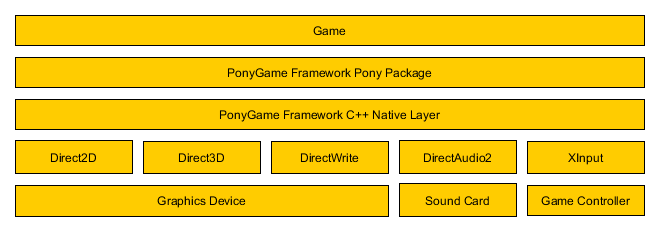
\includegraphics[width=3.5in]{PonyGame.png}
\caption{Architecture of the PonyGame framework.}
\label{fig_ponygame_architecture}
\end{figure}


\section{Actors}
\emph{Actors} in Pony are similar to classes in most object-oriented languages.
However, actors can define \emph{behaviours}, which behave like asynchronous
functions. When you call a behaviour, its body is not executed immediately, but
at some indeterminate time in the future. Like functions, behaviours can have
parameters, but they cannot provide a return value.

With behaviours being executed asynchronously, many behaviours can run at the
same time. The Pony runtime provides an own scheduler, which by default uses a
number of threads equal to the number of CPU cores on the target machine. Each
scheduler thread can be executing an actor behaviour at any given time, making
Pony programs naturally concurrent.

Because of the real-time nature of games, Pony behaviours are ideal candidates
for performing time-consuming tasks that normally would slow down overall game 
performance and degrade user experience, such as writing verbose log files or
computing shortest paths.

While the idea of multi-threading in games isn't new, Pony's \emph{behaviours}
in conjunction with its \emph{reference capabilities} make it easy to develop
games and get all of the message passing and synchronization right. Pony
introduces the concept of \emph{isolated} data structures (\texttt{iso} in Pony)
in addition to the idea of \emph{immutable} data structures in other languages
(e.g. \texttt{const} in C++ or C\#). The notion of isolated data allows actors
to change that data however they like and give it to another actor, which may
(or may not) reside in a different thread.


\section{Memory Management}
Games tend to utilize system memory to the very last bit. For this reason, most
games create their own memory management system. These systems usually use a
combination of multiple prediction algorithms to be able to unload graphics
and sounds when they are no longer needed, and preload others before they are
actually needed in order to prevent hiccups during gameplay.

Others rely on garbage collection of their underlying runtime, such
as Mono, which in turn can be hard to get right: Automatic garbage collection
tends to kick in when least desired, causing performance hits and degrading
user experience.

\emph{Pony-ORCA} is a fully concurrent protocol for garbage collection in the
actor paradigm. It allows cheap and small actors to perform garbage collection
concurrently with any number of other actors, thus preventing the dreaded
\emph{"stop-the-world garbage collection"}.
An actor may perform garbage collection concurrently with other
actors while they are executing any kind of behaviour. Actors reference
isolated data, only. Thus, an actor may decide whether to garbage collect an
object solely based on its own local state - without consulting, or
inspecting the state of, any other actor.


\begin{thebibliography}{1}

\bibitem{CoDesigningATypeSystemAndARuntime}
S.~Clebsch, \emph{Pony: Co-Designing a Type System and a Runtime}.
Microsoft Research, Cambridge, 2016.

\bibitem{PonyTutorial}
S.~T~Allen, S.~Clebsch, S.~Blessing, A.~McNeil et al., \emph{Pony Tutorial}.
\url{http://tutorial.ponylang.org}, 2016.

\bibitem{GarbageCollectionintheActorWorld}
S.~Clebsch, S.~Blessing, J.~Franco, S.~Drossopoulou, \emph{Ownership and
Reference Counting based Garbage Collection in the Actor World}.
Causality Ltd. and Imperial College London, 2015.

\bibitem{GarbageCollectionInTheActorWorld}
S.~Clebsch, S.~Blessing, J.~Franco, S.~Drossopoulou, \emph{Ownership and
Reference Counting based Garbage Collection in the Actor World}. Causality
and Imperial College London, 2015.

\bibitem{FullyConcurrentGarbageCollection}
S.~Clebsch, S.~Drossopoulou, \emph{Fully Concurrent Garbage Collection of
Actors on Many-Core Machines}. OOPSLA 2013.

\bibitem{GarbageCollectionintheActorWorld}
S.~Clebsch, S.~Drossopoulou, S.~Blessing, A.~McNeil, \emph{Deny Capabilities
for Safe, Fast Actors}. Causality Ltd. and Imperial College London.

\end{thebibliography}

\end{document}
